% article with standard layout
\documentclass{beamer}
\usetheme{Darmstadt}

% fancy progress bar
\usepackage{tikz}
\usetikzlibrary{calc}

\definecolor{pbblue}{HTML}{0A75A8}% filling color for the progress bar
\definecolor{pbgray}{HTML}{575757}% background color for the progress bar

\makeatletter
\def\progressbar@progressbar{} % the progress bar
\newcount\progressbar@tmpcounta% auxiliary counter
\newcount\progressbar@tmpcountb% auxiliary counter
\newdimen\progressbar@pbht %progressbar height
\newdimen\progressbar@pbwd %progressbar width
\newdimen\progressbar@tmpdim % auxiliary dimension

\progressbar@pbwd=\linewidth
\progressbar@pbht=1.5ex

% the progress bar
\def\progressbar@progressbar{%

    \progressbar@tmpcounta=\insertframenumber
    \progressbar@tmpcountb=\inserttotalframenumber
    \progressbar@tmpdim=\progressbar@pbwd
    \multiply\progressbar@tmpdim by \progressbar@tmpcounta
    \divide\progressbar@tmpdim by \progressbar@tmpcountb

  \begin{tikzpicture}[rounded corners=2pt,very thin]

    \shade[top color=pbgray!20,bottom color=pbgray!20,middle color=pbgray!50]
      (0pt, 0pt) rectangle ++ (\progressbar@pbwd, \progressbar@pbht);

      \shade[draw=pbblue,top color=pbblue!50,bottom color=pbblue!50,middle color=pbblue] %
        (0pt, 0pt) rectangle ++ (\progressbar@tmpdim, \progressbar@pbht);

    \draw[color=normal text.fg!50]  
      (0pt, 0pt) rectangle (\progressbar@pbwd, \progressbar@pbht) 
        node[pos=0.5,color=normal text.fg] {\textnormal{%
             \pgfmathparse{\insertframenumber*100/\inserttotalframenumber}%
             \pgfmathprintnumber[fixed,precision=2]{\pgfmathresult}\,\%%
        }%
    };
  \end{tikzpicture}%
}

\addtobeamertemplate{footline}{}
{%
  \begin{beamercolorbox}[wd=\paperwidth,ht=4ex,center,dp=1ex]{white}%
    \progressbar@progressbar%
  \end{beamercolorbox}%
}
\makeatother





%encoding text
\usepackage[utf8]{inputenc}
\usepackage[german]{babel}

%biblilatlateography package
\usepackage{csquotes}
\usepackage[backend = biber]{biblatex} 



% fonds
\usepackage[T1]{fontenc}
\usefonttheme{professionalfonts} % using non standard fonts for beamer
\usefonttheme{serif} % default family is serif
%\setmainfont{Liberation Serif}

\usepackage{upgreek}

% math formulas
\usepackage{amsmath}	% standard math equations
%\usepackage[fleqn]{amsmath} % left aligned equations
\usepackage{amsfonts}
\usepackage{amssymb}
\usepackage{amsthm}		% theorem environments
\usepackage{nicefrac}	% make nicefracs ( 1/2 with smaller slash )

% math fond
\usepackage{fourier}

% fancy layout
\usepackage{tcolorbox}

%graphics
\usepackage{graphicx}
\usepackage{wrapfig}
\usepackage{pgfplots} % to simply input matplotlib results

%tables
\usepackage{booktabs}

%layout
\setlength{\parindent}{0pt}
\beamertemplatenavigationsymbolsempty %gets rid of navigation symbols
%\setbeamertemplate{footline}{}  %gets rid of bottom navigation bars

\begin{document}

\title{Structural Error Estimation in Dynamic Systems}
\date{\today}

\maketitle

\begin{frame}{Dynamische Systeme}
	Die zeitliche Entwicklung biologischer Systeme wird durch fundamentale oder empirische Gesetze bestimmt. \\
	\pause
	
	Reale Systeme sind \pause
	\begin{itemize}
	\item[$\to$] offen, \pause
	\item[$\to$] zu komplex, \pause
	\item[$\to$] experimentell nur teilweise zugänglich. \pause
	\end{itemize}
	Vereinfachte Beschreibung durch \textit{dynamische Systeme}
	\begin{equation}
	\frac{\text{d}}{\text{d}\, t} x = f(x,u)  \quad y=h(x) \quad .
	\end{equation}
	Zustand $x$, Observable $y$, Steuerung $u$, Modell $f$.
\end{frame}

\begin{frame}{Dynamic Elastic Net}
	Dynamische Systeme sind unvollständig. \pause
	\begin{table}[h]
		\centering
		\begin{tabular}{lcl}
			nominales Modell &  & wahres Modell \\ \\
			beste Theorie $\tilde{f}$  &\textsf{vs.} & unbekanntes $f$ \\
			simulierte Zustände $\tilde{x}$ &$\longleftrightarrow$ & unbekannte Zustände $x$ \\
			simuliertes $y=h(\tilde{x})$ & & Messwerte $y^\text{data}$			
		\end{tabular}
	\end{table} \pause
	Kann der Fehler des nominalen Modells aus den Daten ermittelt werden? \pause
	\begin{equation}
	w:= f(x,u)- \tilde{f}(x,u)
	\end{equation}
	Kann der \textit{Systemfehler} oder \textit{hidden input} $w$ eindeutig bestimmt werden? 
\end{frame}

\begin{frame}{Lineare Systeme}
	\pause
	Können verschiedene hidden inputs $w$, $w'$ die gleichen Ergebnisse liefern?
	\begin{equation}
	\dot{x} = Ax + Bu + Dw \quad ,\quad \dot{x}' = Ax' + Bu + Dw' \quad \text{sodass} \quad Cx \equiv Cx'
	\end{equation} \pause
	Unter welchen Bedingungen ist die lineare Abbildung
	\begin{equation}
	w \mapsto y = \int\limits_0^{t} C\text{e}^{A(t-\tau)} D w(\tau) \, \text{d}\tau
	\end{equation}
	injektiv?
\end{frame}

\begin{frame}{Beobachtbarkeit}
	Was ist das Urbild von $y\equiv 0$ ? \pause
	\begin{equation}
	y^{(q+1)}(t) = CA^{q+1} \int\limits_0^t \text{e}^{A(t-\tau)}Dw(\tau)\,\text{d}\tau + \sum\limits_{l=0}^q
	CA^lD w^{(q-l)}(t)
	\end{equation} \pause
	Wenn $y\equiv 0$, dann jede Ableitung $y^{(q)}\equiv 0$, d.h. \pause
	\begin{equation}
	\left[ (CD) \, (CAD) \, (CA^2D)\,\ldots \, (CA^qD) \right] \begin{bmatrix}
	w^{(q)}(0) \\ w^{(q-1)}(0) \\ \vdots \\ w^{(0)}(0)
	\end{bmatrix} = 0 \quad \forall q\in\mathbb{N}_0
	\end{equation}
\end{frame}

\begin{frame}{Definitionen} 
	\pause
	\begin{equation}
		\left.
		\begin{aligned}
		M_q &:=\left[ (CD) \, (CAD) \, (CA^2D)\,\ldots \, (CA^qD) \right]\\ 
		V_q &:= \text{ker} M_q 	\\
		W^{(q)} &:= \begin{bmatrix} w^{(q)} , w^{(q-1)}, \hdots , w^{(0)}\end{bmatrix}^\text{T} 
		\end{aligned} \right\} \pause
		\quad \Rightarrow \quad  W^{(q)}(0)\in V_q 
	\end{equation}
	\pause
	\begin{equation} 
		\left.
		\begin{aligned}
		P&: W^{(q)}\mapsto W^{(q-1)} \\ 
		\mathfrak{O}_d &:= V_d \cap P V_{d+1} \cap P^2 V_{d+2} \cap \ldots  	\\
		\end{aligned} \right\} \pause
		\quad \text{damit auch}\quad  W^{(q)}(0)\in \mathfrak{O}_q 
	\end{equation}
\end{frame}

\begin{frame}{Hinreichende Bedingung}
	$\mathfrak{O}_d$ kann in endlich vielen Schritten bestimmt werden, 
	\begin{equation}
	\exists \quad N \in \mathbb{N}_0 \quad \text{sodass} \quad V_d \cap PV_{d+1} \cap \ldots \cap P^NV_{d+N} = 
	\mathfrak{O}_d \quad .
	\end{equation} \pause
	\begin{equation}
	M_q\begin{bmatrix} w^{(q)}(0) \\ \vdots \\w^{(1)}(0) \\ 0 \end{bmatrix} = 
	M_{q-1}\begin{bmatrix} w^{(q)}(0) \\ \vdots \\
	w^{(1)}(0) \end{bmatrix}
	\end{equation}
	
	\begin{block}{Hinreichende Bedingung}
	Falls ein $\mathfrak{O}_d=\{0\}$, dann alle $w^{(q)}(0) = 0$ .
	\end{block} 
	
\end{frame}

\begin{frame}{Notwendige Bedingung}
	\pause
	\begin{equation} \left.
	\begin{aligned}
		\mathfrak{V}_0 &:= V_0\backslash \{0\} \\
		\mathfrak{V}_d &:= V_i \cap P^{-1}\mathfrak{V}_{d-1}
	\end{aligned}\right\} 
	\end{equation} \pause
	\begin{block}{Hinreichende Bedingung}
		Genau dann, wenn alle $\mathfrak{V}_d \neq \emptyset$, existiert eine $\mathbb{R}^m$-wertige Folge 
		$(v_k)_{k\in\mathbb{N}_0}$ mit
		\begin{equation}
		\left[v_k,v_{k-1},\ldots , v_0 \right]^\text{T} \in V_k  \quad \forall k \in \mathbb{N}_0 \quad .
		\end{equation}
	\end{block} \pause
	Dann ist
	\begin{equation}
	w(t) := \sum\limits_{k=0}^\infty \frac{t^k}{k!} v_k 
	\end{equation}
	ein hidden input mit $y^{q}(0)=0$.
\end{frame}

\begin{frame}{Beobachtbarkeit}
	\begin{block}{Lemma}
	$\quad \quad \exists \mathfrak{O}_d=\{0\} \quad \Rightarrow \quad \exists \mathfrak{V}_k = \emptyset$
	\end{block}
	\pause
	Annahme: $w$ kann (stückweise) durch die Taylor-Entwicklung dargestellt werden.\\
	\pause
	Wenn es ein $\mathfrak{V}_d = \emptyset$ gibt, dann gilt
	\begin{equation}
	y\equiv 0 \quad \Longrightarrow \quad w\equiv 0 \quad .
	\end{equation}
\end{frame}

\begin{frame}{Graphische Kriterien} 
	\pause
	\begin{columns}[T]
	\begin{column}{.48\textwidth}
	Der $\alpha$-te hidden input $w_\alpha$ beeinflusst Knoten $x_a$, \\
	die $\beta$-te observable $y_\beta$ hängt von $x_b$ ab. \pause
	\begin{equation*}
	\begin{aligned}
	(CA^kD)_{\beta\alpha} \neq 0 \quad \Leftrightarrow \quad &\exists \text{ Pfad } x_a\to x_b \\ & \text{ der 
	Länge }k  
	\end{aligned}	
	\end{equation*}
	\pause
	Welche Struktur	müssen die $M_q$ besitzen, um
	$\mathfrak{O}_d$ zu garantieren?\\
	\pause
	\tiny{Idee:\\ Zu einem gemessener Knoten $x_\text{obs}$ gibt es Pfade von $\{w_{\alpha_1},w_{\alpha_2},
	\ldots\}$. Von diesen aus gibt es Pfade nach $\{x_{\beta_1},x_{\beta_2},\ldots\}$, usw. 
	Wenn es in diesen Mengen am Ende mehr Observablen als hidden inputs gibt, ist das System observabel? }
	\end{column}\hfill
	\begin{column}{.48\textwidth}
	\begin{figure}[h]
		\centering
		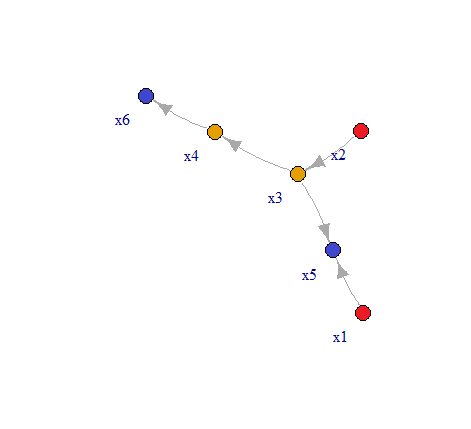
\includegraphics[scale=0.5]{bilder/Sufficient1_Graph.png}
	\end{figure}
	\end{column}
	\end{columns}
\end{frame}

\begin{frame}{Ausblick}
	\begin{enumerate}
	\item Notwendige und hinreichende Bedingungen mit Simulationen abgleichen. (Kann die Wahl eines Algorithmus 
	die Beobachtbarkeit einschränken?) \pause
	\item Kann Regularisierung die Beobachtbarkeit verbessern?\pause
	\item Können graphische Bedingungen formuliert werden? \pause
	\item Können die Ergebnisse im experimental Design angewendet werden? \pause
	\item Wie verhalten sich nichtlineare Systeme? (Gelten die graphischen Bedingungen trotzdem?) \pause
	\end{enumerate}
\end{frame}
\end{document}